\documentclass{article}
\usepackage{graphicx}
\usepackage{color}
\usepackage[small, labelfont = bf]{caption}
\usepackage{epstopdf}
% \usepackage[hypcap = false]{caption} % to add user defined captions

\begin{document}

\begin{center}
    \huge{gnuplot Color, Point and Line Test}
    \vspace{10mm}
\end{center}

\section{gnuplot Test}

    This file shows the values for color and line and point style that are being used in this code. Note that this for terminal \textit{epslatex}. 

\vspace{\fill}
\begin{figure*}[h]
	\centering
% 	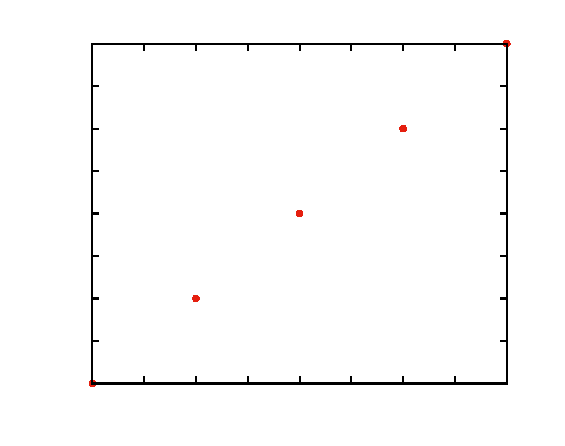
\includegraphics{test_plot}
	\scalebox{0.85}{% GNUPLOT: LaTeX picture with Postscript
\begingroup
  \makeatletter
  \providecommand\color[2][]{%
    \GenericError{(gnuplot) \space\space\space\@spaces}{%
      Package color not loaded in conjunction with
      terminal option `colourtext'%
    }{See the gnuplot documentation for explanation.%
    }{Either use 'blacktext' in gnuplot or load the package
      color.sty in LaTeX.}%
    \renewcommand\color[2][]{}%
  }%
  \providecommand\includegraphics[2][]{%
    \GenericError{(gnuplot) \space\space\space\@spaces}{%
      Package graphicx or graphics not loaded%
    }{See the gnuplot documentation for explanation.%
    }{The gnuplot epslatex terminal needs graphicx.sty or graphics.sty.}%
    \renewcommand\includegraphics[2][]{}%
  }%
  \providecommand\rotatebox[2]{#2}%
  \@ifundefined{ifGPcolor}{%
    \newif\ifGPcolor
    \GPcolortrue
  }{}%
  \@ifundefined{ifGPblacktext}{%
    \newif\ifGPblacktext
    \GPblacktextfalse
  }{}%
  % define a \g@addto@macro without @ in the name:
  \let\gplgaddtomacro\g@addto@macro
  % define empty templates for all commands taking text:
  \gdef\gplbacktext{}%
  \gdef\gplfronttext{}%
  \makeatother
  \ifGPblacktext
    % no textcolor at all
    \def\colorrgb#1{}%
    \def\colorgray#1{}%
  \else
    % gray or color?
    \ifGPcolor
      \def\colorrgb#1{\color[rgb]{#1}}%
      \def\colorgray#1{\color[gray]{#1}}%
      \expandafter\def\csname LTw\endcsname{\color{white}}%
      \expandafter\def\csname LTb\endcsname{\color{black}}%
      \expandafter\def\csname LTa\endcsname{\color{black}}%
      \expandafter\def\csname LT0\endcsname{\color[rgb]{1,0,0}}%
      \expandafter\def\csname LT1\endcsname{\color[rgb]{0,1,0}}%
      \expandafter\def\csname LT2\endcsname{\color[rgb]{0,0,1}}%
      \expandafter\def\csname LT3\endcsname{\color[rgb]{1,0,1}}%
      \expandafter\def\csname LT4\endcsname{\color[rgb]{0,1,1}}%
      \expandafter\def\csname LT5\endcsname{\color[rgb]{1,1,0}}%
      \expandafter\def\csname LT6\endcsname{\color[rgb]{0,0,0}}%
      \expandafter\def\csname LT7\endcsname{\color[rgb]{1,0.3,0}}%
      \expandafter\def\csname LT8\endcsname{\color[rgb]{0.5,0.5,0.5}}%
    \else
      % gray
      \def\colorrgb#1{\color{black}}%
      \def\colorgray#1{\color[gray]{#1}}%
      \expandafter\def\csname LTw\endcsname{\color{white}}%
      \expandafter\def\csname LTb\endcsname{\color{black}}%
      \expandafter\def\csname LTa\endcsname{\color{black}}%
      \expandafter\def\csname LT0\endcsname{\color{black}}%
      \expandafter\def\csname LT1\endcsname{\color{black}}%
      \expandafter\def\csname LT2\endcsname{\color{black}}%
      \expandafter\def\csname LT3\endcsname{\color{black}}%
      \expandafter\def\csname LT4\endcsname{\color{black}}%
      \expandafter\def\csname LT5\endcsname{\color{black}}%
      \expandafter\def\csname LT6\endcsname{\color{black}}%
      \expandafter\def\csname LT7\endcsname{\color{black}}%
      \expandafter\def\csname LT8\endcsname{\color{black}}%
    \fi
  \fi
    \setlength{\unitlength}{0.0500bp}%
    \ifx\gptboxheight\undefined%
      \newlength{\gptboxheight}%
      \newlength{\gptboxwidth}%
      \newsavebox{\gptboxtext}%
    \fi%
    \setlength{\fboxrule}{0.5pt}%
    \setlength{\fboxsep}{1pt}%
\begin{picture}(8502.00,6236.00)%
    \gplgaddtomacro\gplfronttext{%
      \csname LTb\endcsname%
      \put(264,6016){\makebox(0,0)[l]{\strut{}epslatex  terminal test}}%
      \put(264,5741){\makebox(0,0)[l]{\strut{}gnuplot version 5.0.1  }}%
      \csname LTb\endcsname%
      \put(2931,3118){\makebox(0,0)[l]{\strut{}12345678901234567890}}%
      \put(2931,3426){\makebox(0,0)[l]{\strut{}test of character width:}}%
      \put(4251,4438){\makebox(0,0)[l]{\strut{}left justified}}%
      \put(4251,4218){\makebox(0,0){\strut{}centre+d text}}%
      \put(4251,3998){\makebox(0,0)[r]{\strut{}right justified}}%
      \csname LT1\endcsname%
      \put(220,3118){\rotatebox{-270}{\makebox(0,0){\strut{}rotated ce+ntred text}}}%
      \put(660,3118){\rotatebox{45}{\makebox(0,0)[l]{\strut{} rotated by +45 deg}}}%
      \put(440,3118){\rotatebox{-45}{\makebox(0,0)[l]{\strut{} rotated by -45 deg}}}%
      \csname LT2\endcsname%
      \put(4119,6016){\makebox(0,0)[r]{\strut{}show ticscale}}%
      \csname LTb\endcsname%
      \put(7515,6016){\makebox(0,0)[r]{\strut{}-1}}%
      \csname LTa\endcsname%
      \put(7515,5796){\makebox(0,0)[r]{\strut{}0}}%
      \colorrgb{0.58,0.00,0.83}%
      \put(7515,5576){\makebox(0,0)[r]{\strut{}1}}%
      \colorrgb{0.00,0.62,0.45}%
      \put(7515,5356){\makebox(0,0)[r]{\strut{}2}}%
      \colorrgb{0.34,0.71,0.91}%
      \put(7515,5136){\makebox(0,0)[r]{\strut{}3}}%
      \colorrgb{0.90,0.62,0.00}%
      \put(7515,4916){\makebox(0,0)[r]{\strut{}4}}%
      \colorrgb{0.94,0.89,0.26}%
      \put(7515,4696){\makebox(0,0)[r]{\strut{}5}}%
      \colorrgb{0.00,0.45,0.70}%
      \put(7515,4476){\makebox(0,0)[r]{\strut{}6}}%
      \colorrgb{0.90,0.12,0.06}%
      \put(7515,4256){\makebox(0,0)[r]{\strut{}7}}%
      \colorrgb{0.00,0.00,0.00}%
      \put(7515,4036){\makebox(0,0)[r]{\strut{}8}}%
      \colorrgb{0.58,0.00,0.83}%
      \put(7515,3816){\makebox(0,0)[r]{\strut{}9}}%
      \colorrgb{0.00,0.62,0.45}%
      \put(7515,3596){\makebox(0,0)[r]{\strut{}10}}%
      \colorrgb{0.34,0.71,0.91}%
      \put(7515,3376){\makebox(0,0)[r]{\strut{}11}}%
      \colorrgb{0.90,0.62,0.00}%
      \put(7515,3156){\makebox(0,0)[r]{\strut{}12}}%
      \colorrgb{0.94,0.89,0.26}%
      \put(7515,2936){\makebox(0,0)[r]{\strut{}13}}%
      \colorrgb{0.00,0.45,0.70}%
      \put(7515,2716){\makebox(0,0)[r]{\strut{}14}}%
      \colorrgb{0.90,0.12,0.06}%
      \put(7515,2496){\makebox(0,0)[r]{\strut{}15}}%
      \colorrgb{0.00,0.00,0.00}%
      \put(7515,2276){\makebox(0,0)[r]{\strut{}16}}%
      \colorrgb{0.58,0.00,0.83}%
      \put(7515,2056){\makebox(0,0)[r]{\strut{}17}}%
      \colorrgb{0.00,0.62,0.45}%
      \put(7515,1836){\makebox(0,0)[r]{\strut{}18}}%
      \colorrgb{0.34,0.71,0.91}%
      \put(7515,1616){\makebox(0,0)[r]{\strut{}19}}%
      \colorrgb{0.90,0.62,0.00}%
      \put(7515,1396){\makebox(0,0)[r]{\strut{}20}}%
      \colorrgb{0.94,0.89,0.26}%
      \put(7515,1176){\makebox(0,0)[r]{\strut{}21}}%
      \colorrgb{0.00,0.45,0.70}%
      \put(7515,956){\makebox(0,0)[r]{\strut{}22}}%
      \colorrgb{0.90,0.12,0.06}%
      \put(7515,736){\makebox(0,0)[r]{\strut{}23}}%
      \colorrgb{0.00,0.00,0.00}%
      \put(7515,516){\makebox(0,0)[r]{\strut{}24}}%
      \colorrgb{0.58,0.00,0.83}%
      \put(7515,296){\makebox(0,0)[r]{\strut{}25}}%
      \csname LTb\endcsname%
      \put(1487,249){\makebox(0,0)[l]{\strut{}  lw 1}}%
      \put(1487,498){\makebox(0,0)[l]{\strut{}  lw 2}}%
      \put(1487,747){\makebox(0,0)[l]{\strut{}  lw 3}}%
      \put(1487,996){\makebox(0,0)[l]{\strut{}  lw 4}}%
      \put(1487,1245){\makebox(0,0)[l]{\strut{}  lw 5}}%
      \put(1487,1494){\makebox(0,0)[l]{\strut{}  lw 6}}%
      \put(637,1743){\makebox(0,0)[l]{\strut{}linewidth}}%
      \put(3400,249){\makebox(0,0)[l]{\strut{}  dt 0}}%
      \csname LTb\endcsname%
      \put(3400,498){\makebox(0,0)[l]{\strut{}  dt 1}}%
      \csname LTb\endcsname%
      \put(3400,747){\makebox(0,0)[l]{\strut{}  dt 2}}%
      \csname LTb\endcsname%
      \put(3400,996){\makebox(0,0)[l]{\strut{}  dt 3}}%
      \csname LTb\endcsname%
      \put(3400,1245){\makebox(0,0)[l]{\strut{}  dt 4}}%
      \put(2550,1494){\makebox(0,0)[l]{\strut{}dashtype}}%
      \put(5735,1109){\makebox(0,0){\strut{}pattern fill}}%
      \put(4357,889){\makebox(0,0){\strut{} 0}}%
      \put(4675,889){\makebox(0,0){\strut{} 1}}%
      \put(4993,889){\makebox(0,0){\strut{} 2}}%
      \put(5311,889){\makebox(0,0){\strut{} 3}}%
      \put(5629,889){\makebox(0,0){\strut{} 4}}%
      \put(5947,889){\makebox(0,0){\strut{} 5}}%
      \put(6265,889){\makebox(0,0){\strut{} 6}}%
      \put(6583,889){\makebox(0,0){\strut{} 7}}%
      \put(6901,889){\makebox(0,0){\strut{} 8}}%
      \csname LTb\endcsname%
      \put(5951,5710){\makebox(0,0){\strut{}filled polygons:}}%
    }%
    \gplbacktext
    \put(0,0){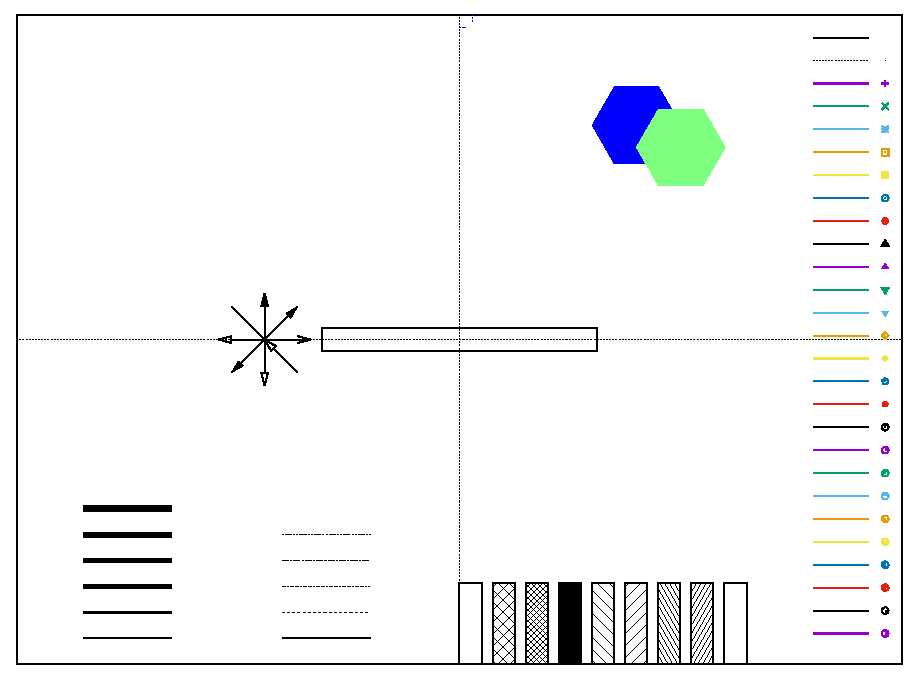
\includegraphics{test_color}}%
    \gplfronttext
  \end{picture}%
\endgroup
}
	\caption{\label{fig:test} Use this for setting the color in \LaTeX.}
\end{figure*}
\vspace{\fill}

\end{document}